\documentclass[11pt]{article}
\usepackage[textwidth=18.0cm, textheight=23.0cm, top=2.0cm]{geometry}
\usepackage{pst-all}
\usepackage{amssymb}
\usepackage{tikz}
\usepackage{underscore}\begin{document}
\pagestyle{empty}


ClassName: \underline{\textbf{Class_08.2bp-15}}
\par
BinSize: \underline{\textbf{100 × 100}}
\par
ReduceSize: \underline{\textbf{100 × 100}}
\par
TypeNum: \underline{\textbf{40}}
\par
Num: \underline{\textbf{40}}
\par
OutS: \underline{\textbf{120000}}
\par
InS: \underline{\textbf{94805}}
\par
Rate: \underline{\textbf{0.790}}
\par
UB: \underline{\textbf{12}}
\par
LB0: \underline{\textbf{12}}
\par
LB: \underline{\textbf{12}}
\par
LBWithCut: \underline{\textbf{12}}
\par
NodeCut: \underline{\textbf{0}}
\par
ExtendedNodeCnt: \underline{\textbf{1}}
\par
GenNodeCnt: \underline{\textbf{1}}
\par
PrimalNode: \underline{\textbf{0}}
\par
ColumnCount: \underline{\textbf{12}}
\par
TotalCutCount: \underline{\textbf{0}}
\par
RootCutCount: \underline{\textbf{0}}
\par
LPSolverCnt: \underline{\textbf{1}}
\par
PricingSolverCnt: \underline{\textbf{0}}
\par
BranchAndBoundNum: \underline{\textbf{1}}
\par
isOpt: \underline{\textbf{true}}
\par
TimeOnInitSolution: \underline{\textbf{600.000 s}}
\par
TimeOnPrimal: \underline{\textbf{0.000 s}}
\par
TimeOnPricing: \underline{\textbf{0.000 s}}
\par
TimeOnRmp: \underline{\textbf{0.063 s}}
\par
TotalTime: \underline{\textbf{600.297 s}}
\par
\newpage


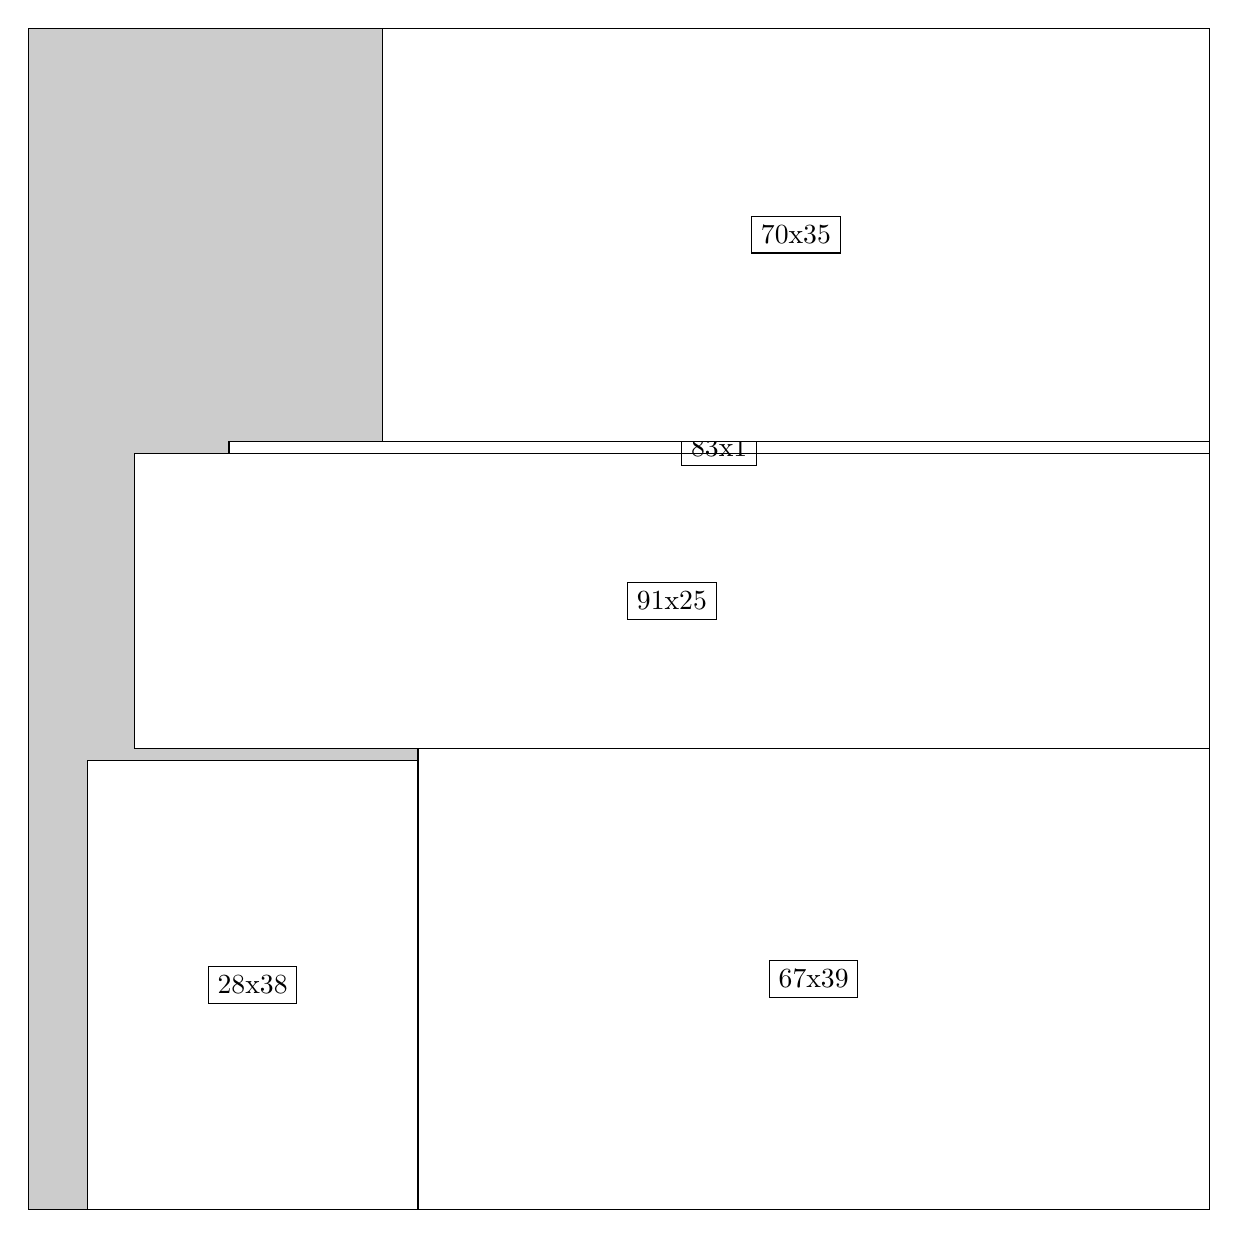
\begin{tikzpicture}[shorten >=1pt,scale=1.0,every node/.style={scale=1.0},->]
\tikzstyle{vertex}=[circle,fill=black!25,minimum size=14pt,inner sep=0pt]
\filldraw[fill=gray!40!white, draw=black] (0,0) rectangle (15.0,15.0);
\foreach \name/\x/\y/\w/\h in {67x39/4.95/0.0/10.049999999999999/5.85,28x38/0.75/0.0/4.2/5.7,91x25/1.3499999999999999/5.85/13.65/3.75,83x1/2.55/9.6/12.45/0.15,70x35/4.5/9.75/10.5/5.25}
\filldraw[fill=white!40!white, draw=black] (\x,\y) rectangle node[draw] (\name) {\name} ++(\w,\h);
\end{tikzpicture}


w =67 , h =39 , x =33 , y =0 , v =2613
\par
w =28 , h =38 , x =5 , y =0 , v =1064
\par
w =91 , h =25 , x =9 , y =39 , v =2275
\par
w =83 , h =1 , x =17 , y =64 , v =83
\par
w =70 , h =35 , x =30 , y =65 , v =2450
\par
\newpage


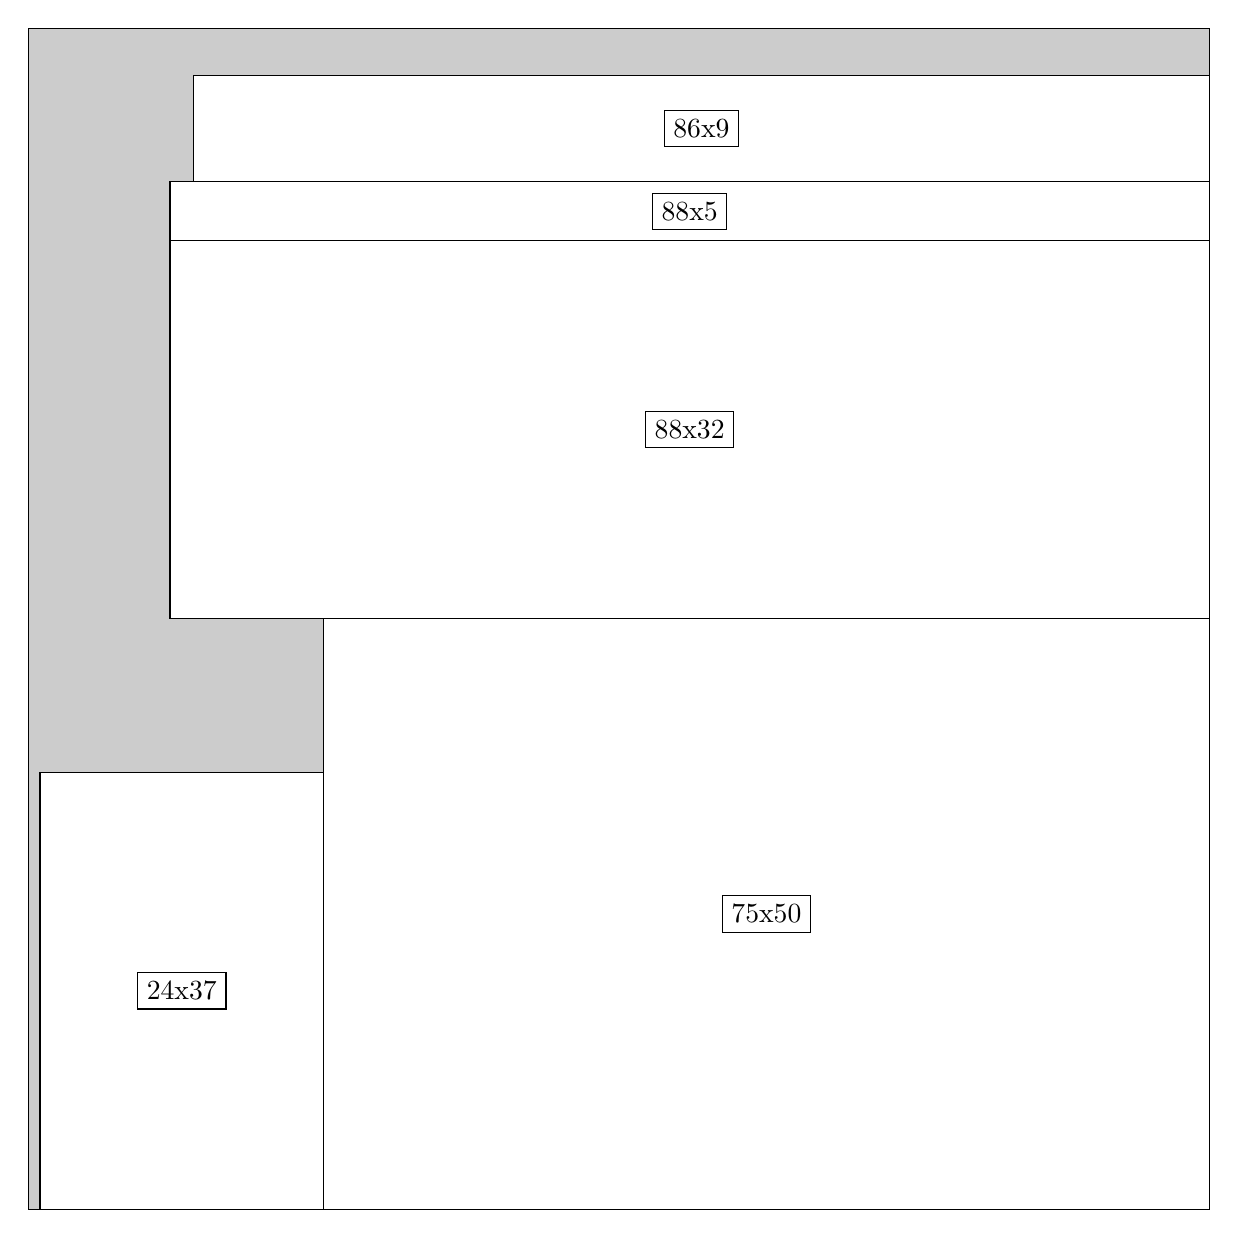
\begin{tikzpicture}[shorten >=1pt,scale=1.0,every node/.style={scale=1.0},->]
\tikzstyle{vertex}=[circle,fill=black!25,minimum size=14pt,inner sep=0pt]
\filldraw[fill=gray!40!white, draw=black] (0,0) rectangle (15.0,15.0);
\foreach \name/\x/\y/\w/\h in {75x50/3.75/0.0/11.25/7.5,24x37/0.15/0.0/3.5999999999999996/5.55,88x32/1.7999999999999998/7.5/13.2/4.8,88x5/1.7999999999999998/12.299999999999999/13.2/0.75,86x9/2.1/13.049999999999999/12.9/1.3499999999999999}
\filldraw[fill=white!40!white, draw=black] (\x,\y) rectangle node[draw] (\name) {\name} ++(\w,\h);
\end{tikzpicture}


w =75 , h =50 , x =25 , y =0 , v =3750
\par
w =24 , h =37 , x =1 , y =0 , v =888
\par
w =88 , h =32 , x =12 , y =50 , v =2816
\par
w =88 , h =5 , x =12 , y =82 , v =440
\par
w =86 , h =9 , x =14 , y =87 , v =774
\par
\newpage


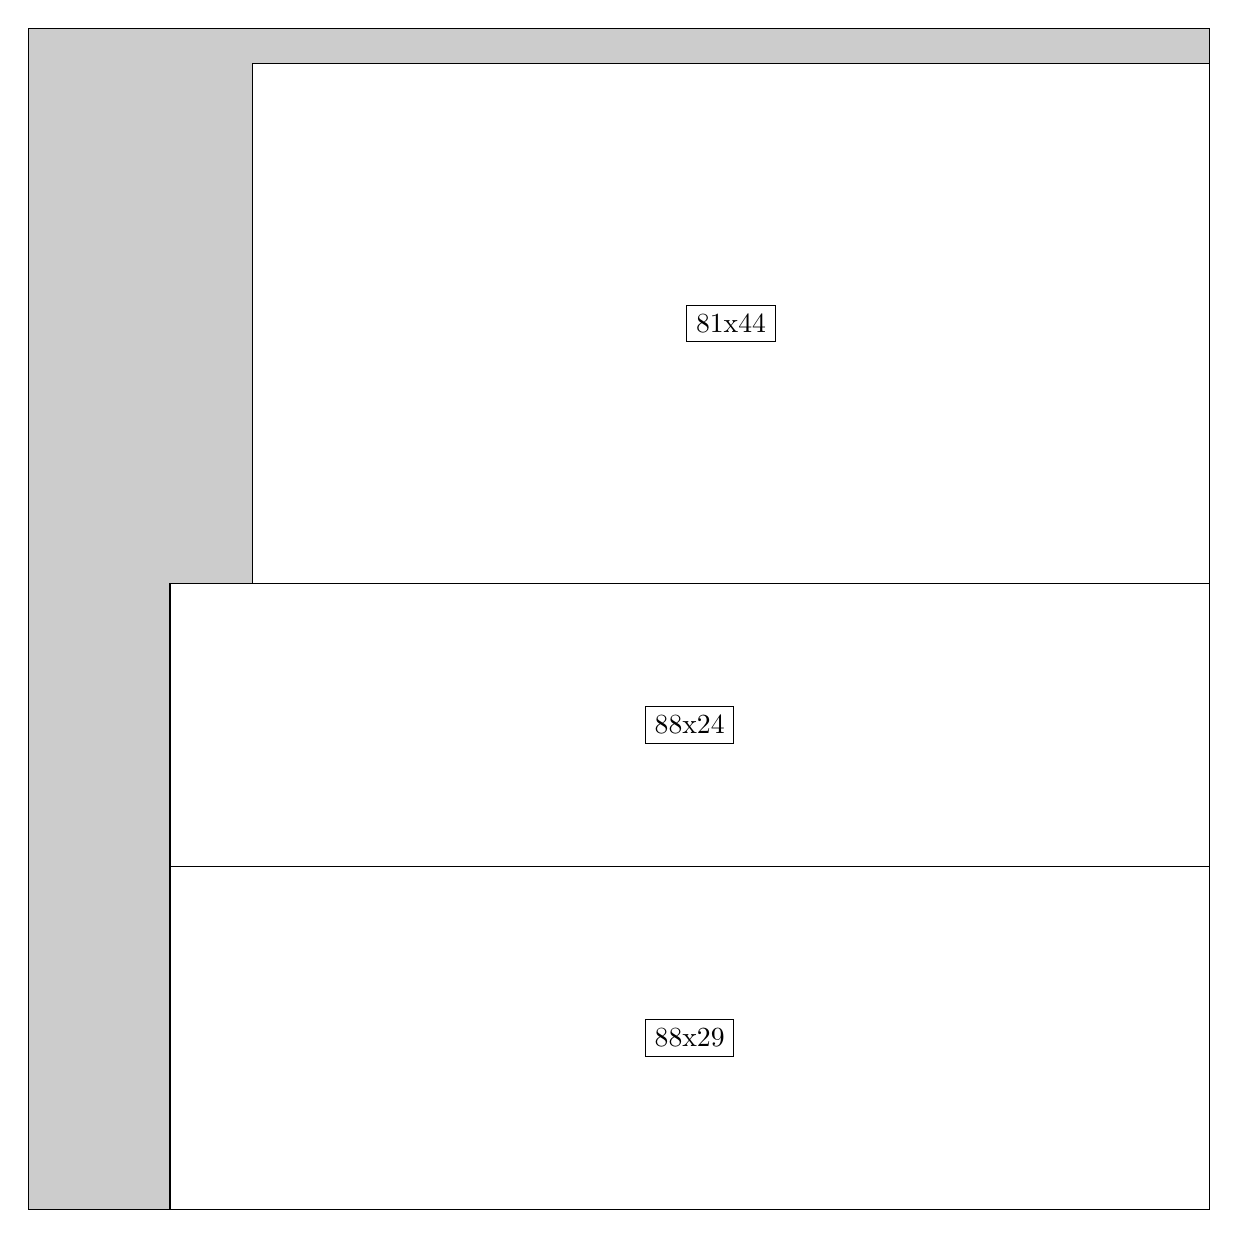
\begin{tikzpicture}[shorten >=1pt,scale=1.0,every node/.style={scale=1.0},->]
\tikzstyle{vertex}=[circle,fill=black!25,minimum size=14pt,inner sep=0pt]
\filldraw[fill=gray!40!white, draw=black] (0,0) rectangle (15.0,15.0);
\foreach \name/\x/\y/\w/\h in {88x29/1.7999999999999998/0.0/13.2/4.35,88x24/1.7999999999999998/4.35/13.2/3.5999999999999996,81x44/2.85/7.949999999999999/12.15/6.6}
\filldraw[fill=white!40!white, draw=black] (\x,\y) rectangle node[draw] (\name) {\name} ++(\w,\h);
\end{tikzpicture}


w =88 , h =29 , x =12 , y =0 , v =2552
\par
w =88 , h =24 , x =12 , y =29 , v =2112
\par
w =81 , h =44 , x =19 , y =53 , v =3564
\par
\newpage


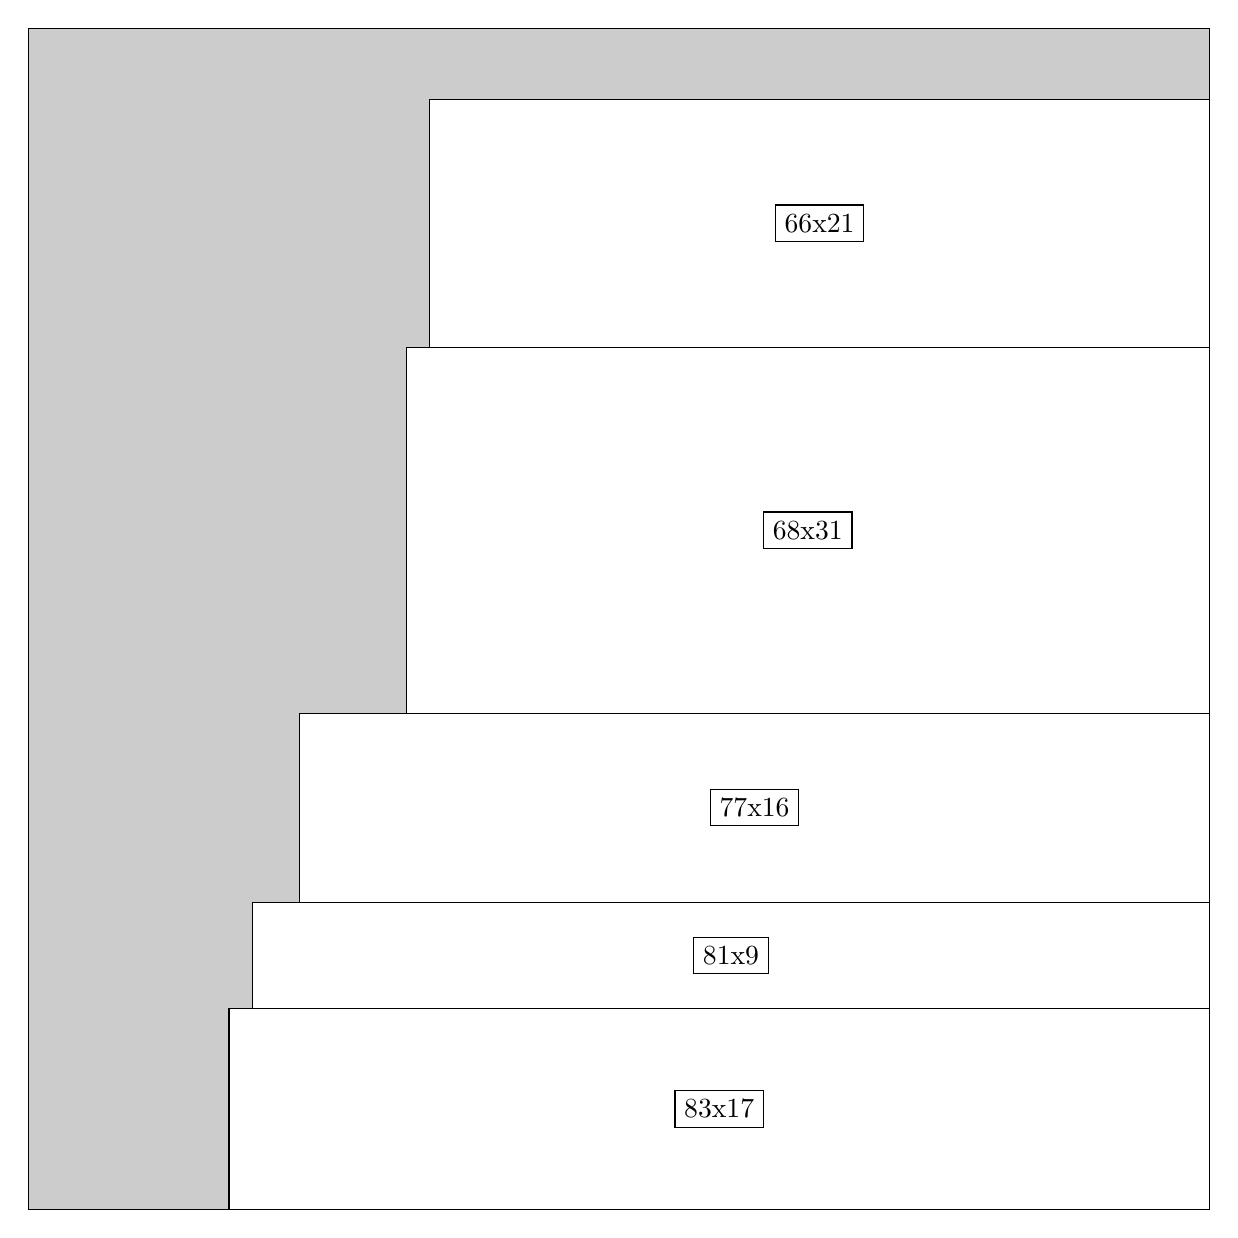
\begin{tikzpicture}[shorten >=1pt,scale=1.0,every node/.style={scale=1.0},->]
\tikzstyle{vertex}=[circle,fill=black!25,minimum size=14pt,inner sep=0pt]
\filldraw[fill=gray!40!white, draw=black] (0,0) rectangle (15.0,15.0);
\foreach \name/\x/\y/\w/\h in {83x17/2.55/0.0/12.45/2.55,81x9/2.85/2.55/12.15/1.3499999999999999,77x16/3.4499999999999997/3.9/11.549999999999999/2.4,68x31/4.8/6.3/10.2/4.6499999999999995,66x21/5.1/10.95/9.9/3.15}
\filldraw[fill=white!40!white, draw=black] (\x,\y) rectangle node[draw] (\name) {\name} ++(\w,\h);
\end{tikzpicture}


w =83 , h =17 , x =17 , y =0 , v =1411
\par
w =81 , h =9 , x =19 , y =17 , v =729
\par
w =77 , h =16 , x =23 , y =26 , v =1232
\par
w =68 , h =31 , x =32 , y =42 , v =2108
\par
w =66 , h =21 , x =34 , y =73 , v =1386
\par
\newpage


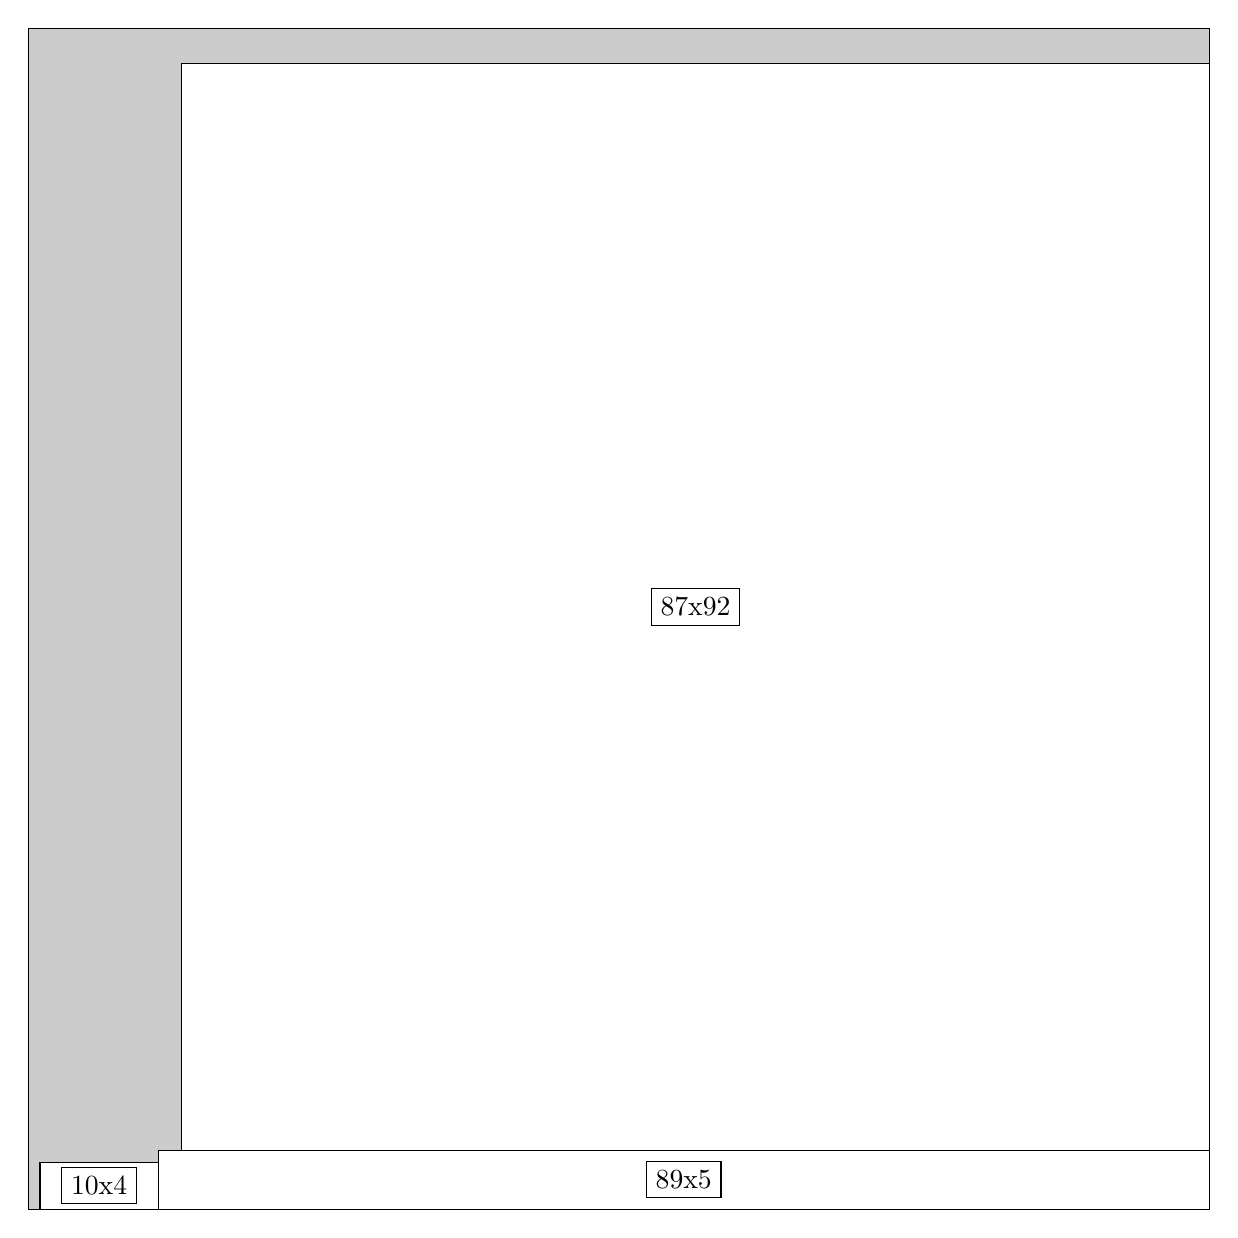
\begin{tikzpicture}[shorten >=1pt,scale=1.0,every node/.style={scale=1.0},->]
\tikzstyle{vertex}=[circle,fill=black!25,minimum size=14pt,inner sep=0pt]
\filldraw[fill=gray!40!white, draw=black] (0,0) rectangle (15.0,15.0);
\foreach \name/\x/\y/\w/\h in {89x5/1.65/0.0/13.35/0.75,10x4/0.15/0.0/1.5/0.6,87x92/1.95/0.75/13.049999999999999/13.799999999999999}
\filldraw[fill=white!40!white, draw=black] (\x,\y) rectangle node[draw] (\name) {\name} ++(\w,\h);
\end{tikzpicture}


w =89 , h =5 , x =11 , y =0 , v =445
\par
w =10 , h =4 , x =1 , y =0 , v =40
\par
w =87 , h =92 , x =13 , y =5 , v =8004
\par
\newpage


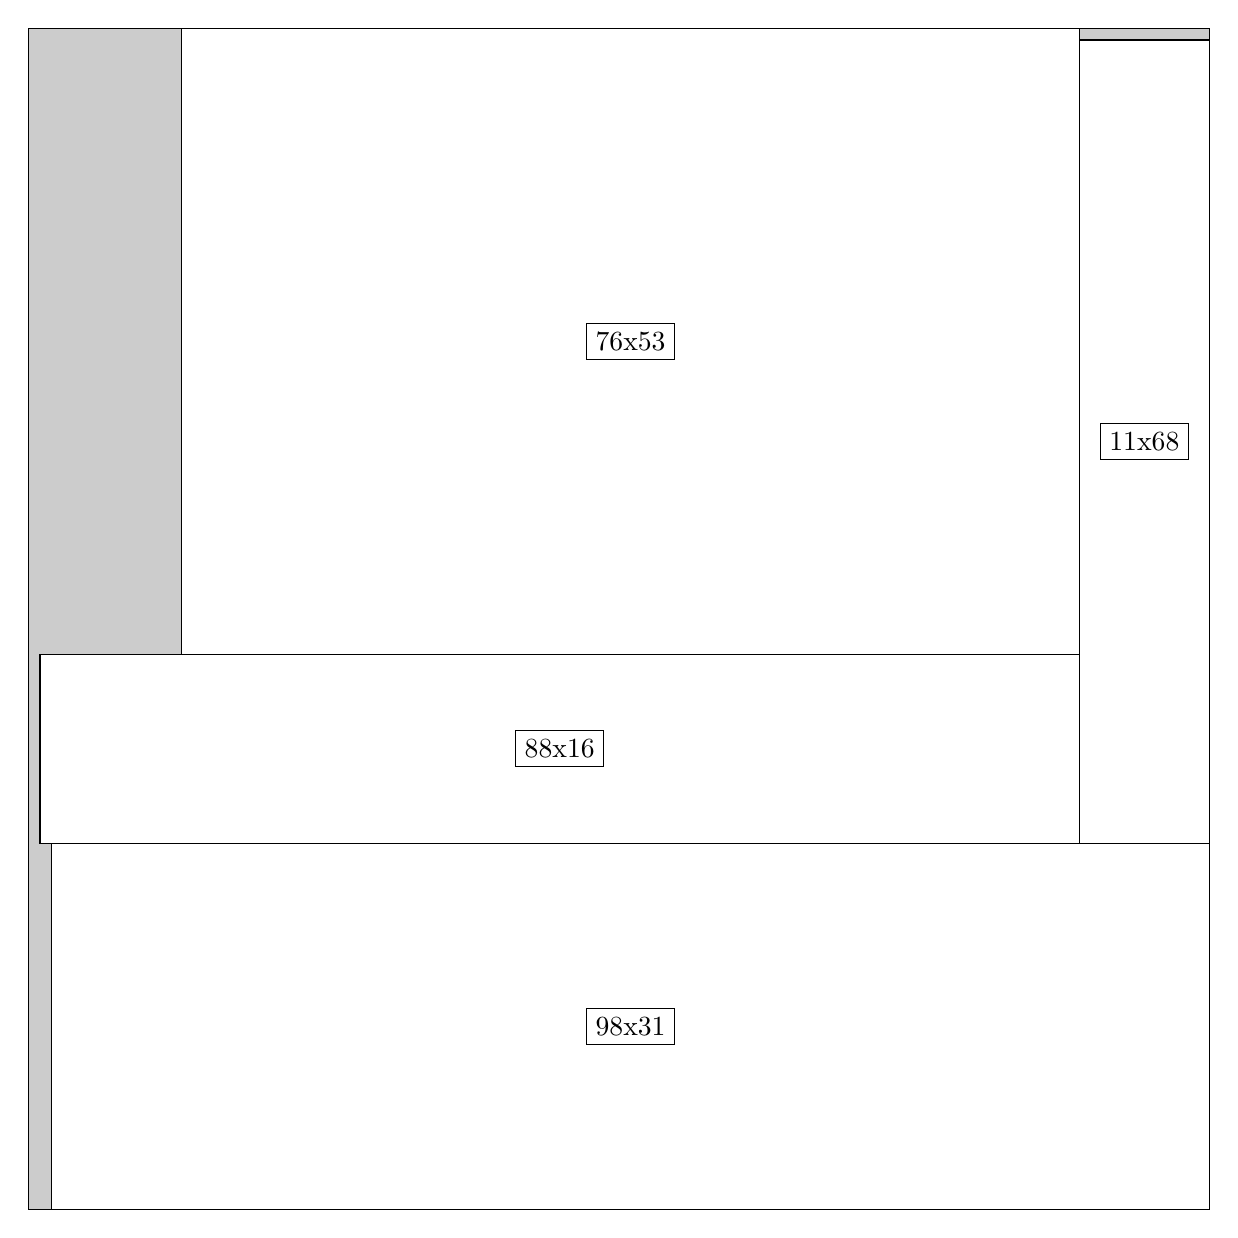
\begin{tikzpicture}[shorten >=1pt,scale=1.0,every node/.style={scale=1.0},->]
\tikzstyle{vertex}=[circle,fill=black!25,minimum size=14pt,inner sep=0pt]
\filldraw[fill=gray!40!white, draw=black] (0,0) rectangle (15.0,15.0);
\foreach \name/\x/\y/\w/\h in {98x31/0.3/0.0/14.7/4.6499999999999995,11x68/13.35/4.6499999999999995/1.65/10.2,88x16/0.15/4.6499999999999995/13.2/2.4,76x53/1.95/7.05/11.4/7.949999999999999}
\filldraw[fill=white!40!white, draw=black] (\x,\y) rectangle node[draw] (\name) {\name} ++(\w,\h);
\end{tikzpicture}


w =98 , h =31 , x =2 , y =0 , v =3038
\par
w =11 , h =68 , x =89 , y =31 , v =748
\par
w =88 , h =16 , x =1 , y =31 , v =1408
\par
w =76 , h =53 , x =13 , y =47 , v =4028
\par
\newpage


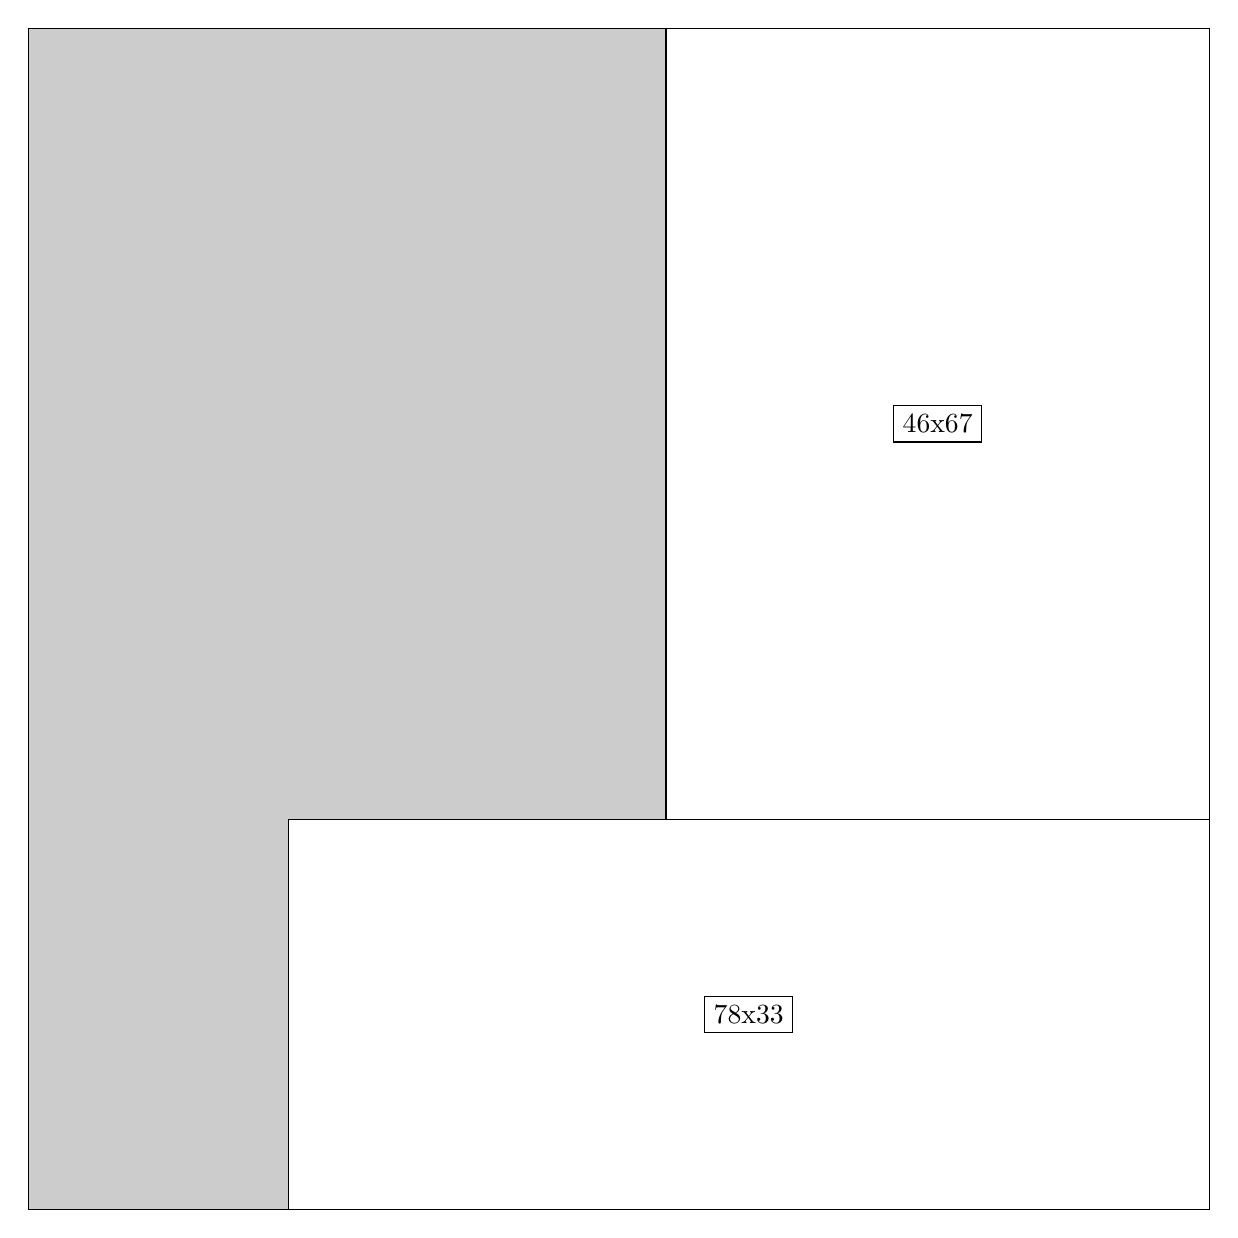
\begin{tikzpicture}[shorten >=1pt,scale=1.0,every node/.style={scale=1.0},->]
\tikzstyle{vertex}=[circle,fill=black!25,minimum size=14pt,inner sep=0pt]
\filldraw[fill=gray!40!white, draw=black] (0,0) rectangle (15.0,15.0);
\foreach \name/\x/\y/\w/\h in {78x33/3.3/0.0/11.7/4.95,46x67/8.1/4.95/6.8999999999999995/10.049999999999999}
\filldraw[fill=white!40!white, draw=black] (\x,\y) rectangle node[draw] (\name) {\name} ++(\w,\h);
\end{tikzpicture}


w =78 , h =33 , x =22 , y =0 , v =2574
\par
w =46 , h =67 , x =54 , y =33 , v =3082
\par
\newpage


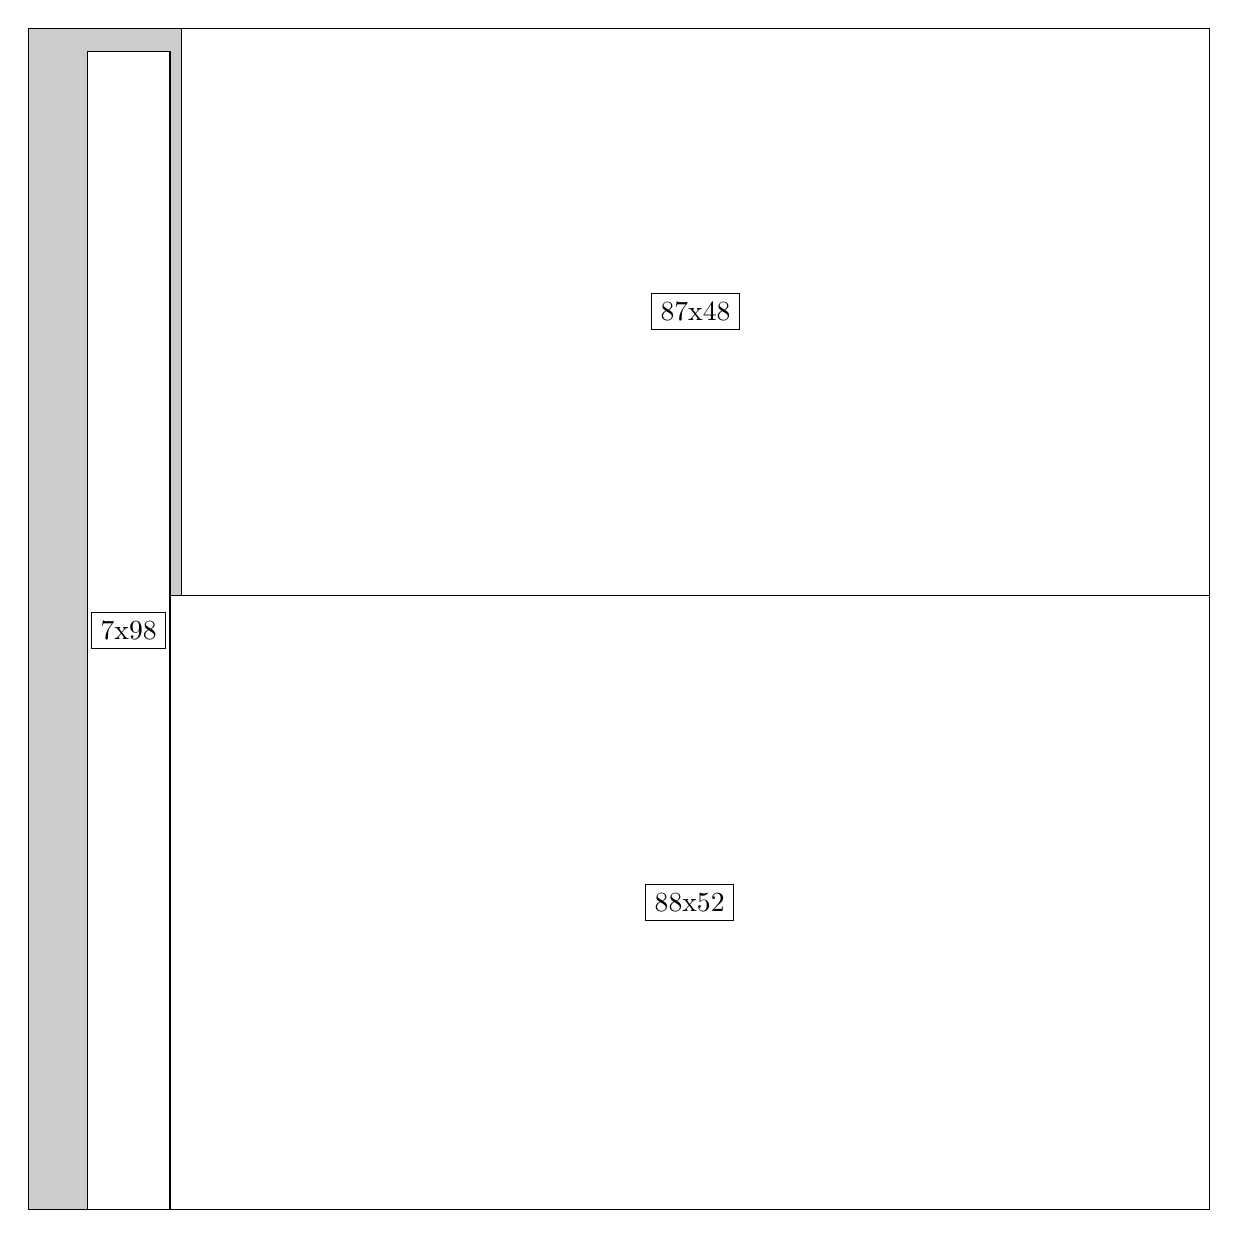
\begin{tikzpicture}[shorten >=1pt,scale=1.0,every node/.style={scale=1.0},->]
\tikzstyle{vertex}=[circle,fill=black!25,minimum size=14pt,inner sep=0pt]
\filldraw[fill=gray!40!white, draw=black] (0,0) rectangle (15.0,15.0);
\foreach \name/\x/\y/\w/\h in {88x52/1.7999999999999998/0.0/13.2/7.8,87x48/1.95/7.8/13.049999999999999/7.199999999999999,7x98/0.75/0.0/1.05/14.7}
\filldraw[fill=white!40!white, draw=black] (\x,\y) rectangle node[draw] (\name) {\name} ++(\w,\h);
\end{tikzpicture}


w =88 , h =52 , x =12 , y =0 , v =4576
\par
w =87 , h =48 , x =13 , y =52 , v =4176
\par
w =7 , h =98 , x =5 , y =0 , v =686
\par
\newpage


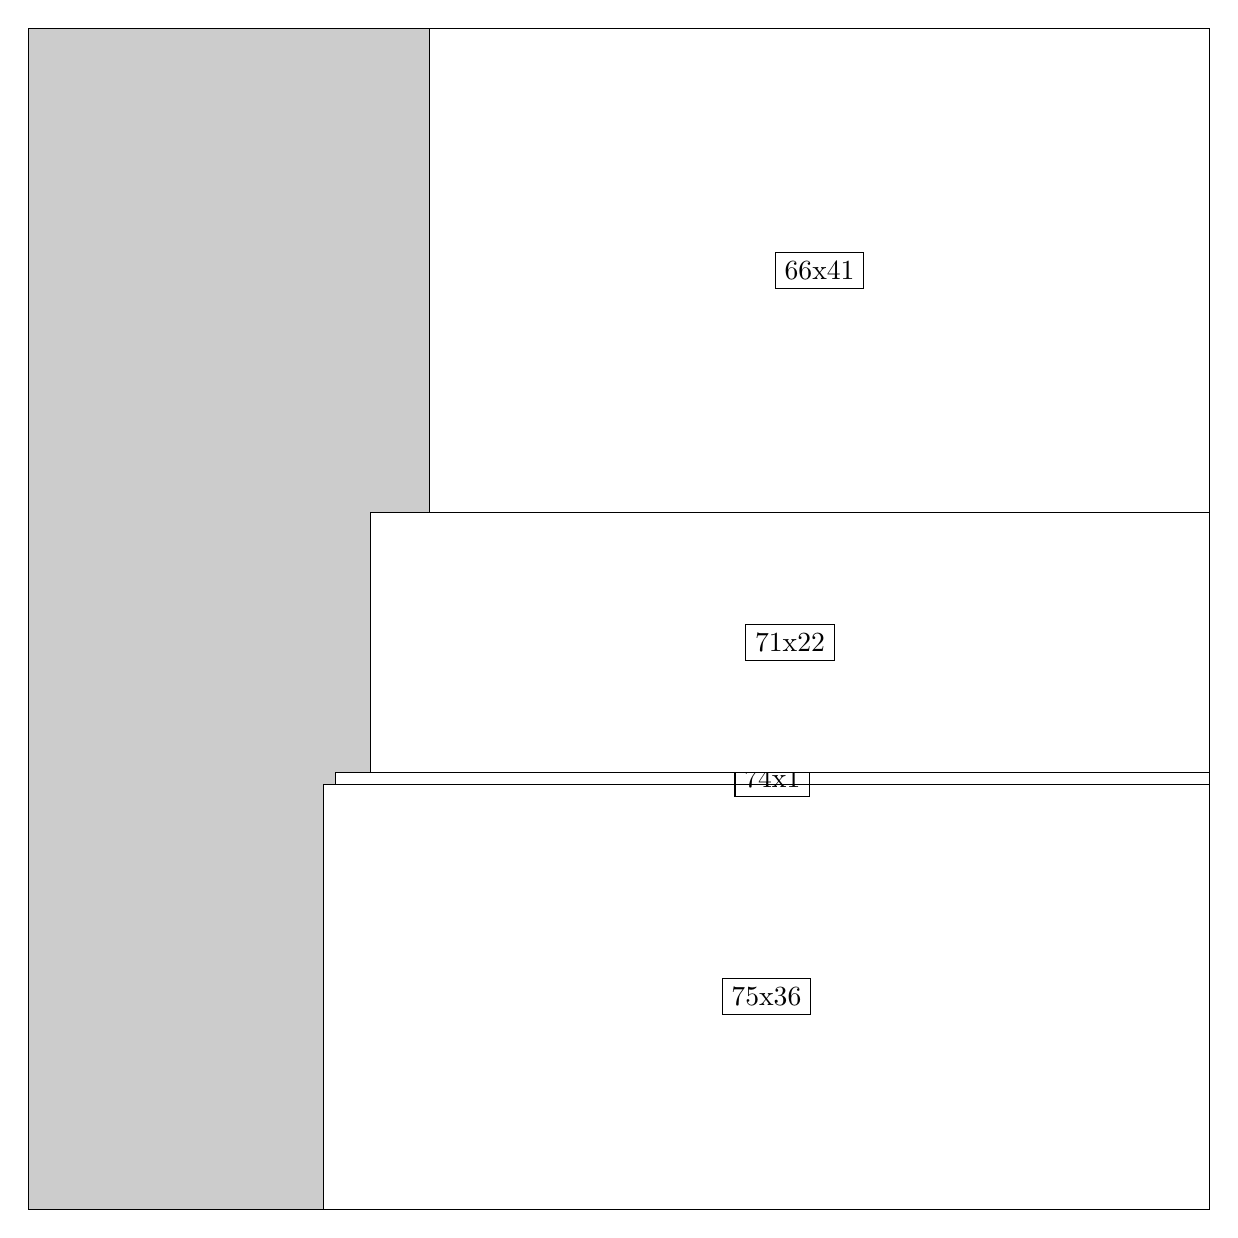
\begin{tikzpicture}[shorten >=1pt,scale=1.0,every node/.style={scale=1.0},->]
\tikzstyle{vertex}=[circle,fill=black!25,minimum size=14pt,inner sep=0pt]
\filldraw[fill=gray!40!white, draw=black] (0,0) rectangle (15.0,15.0);
\foreach \name/\x/\y/\w/\h in {75x36/3.75/0.0/11.25/5.3999999999999995,74x1/3.9/5.3999999999999995/11.1/0.15,71x22/4.35/5.55/10.65/3.3,66x41/5.1/8.85/9.9/6.1499999999999995}
\filldraw[fill=white!40!white, draw=black] (\x,\y) rectangle node[draw] (\name) {\name} ++(\w,\h);
\end{tikzpicture}


w =75 , h =36 , x =25 , y =0 , v =2700
\par
w =74 , h =1 , x =26 , y =36 , v =74
\par
w =71 , h =22 , x =29 , y =37 , v =1562
\par
w =66 , h =41 , x =34 , y =59 , v =2706
\par
\newpage


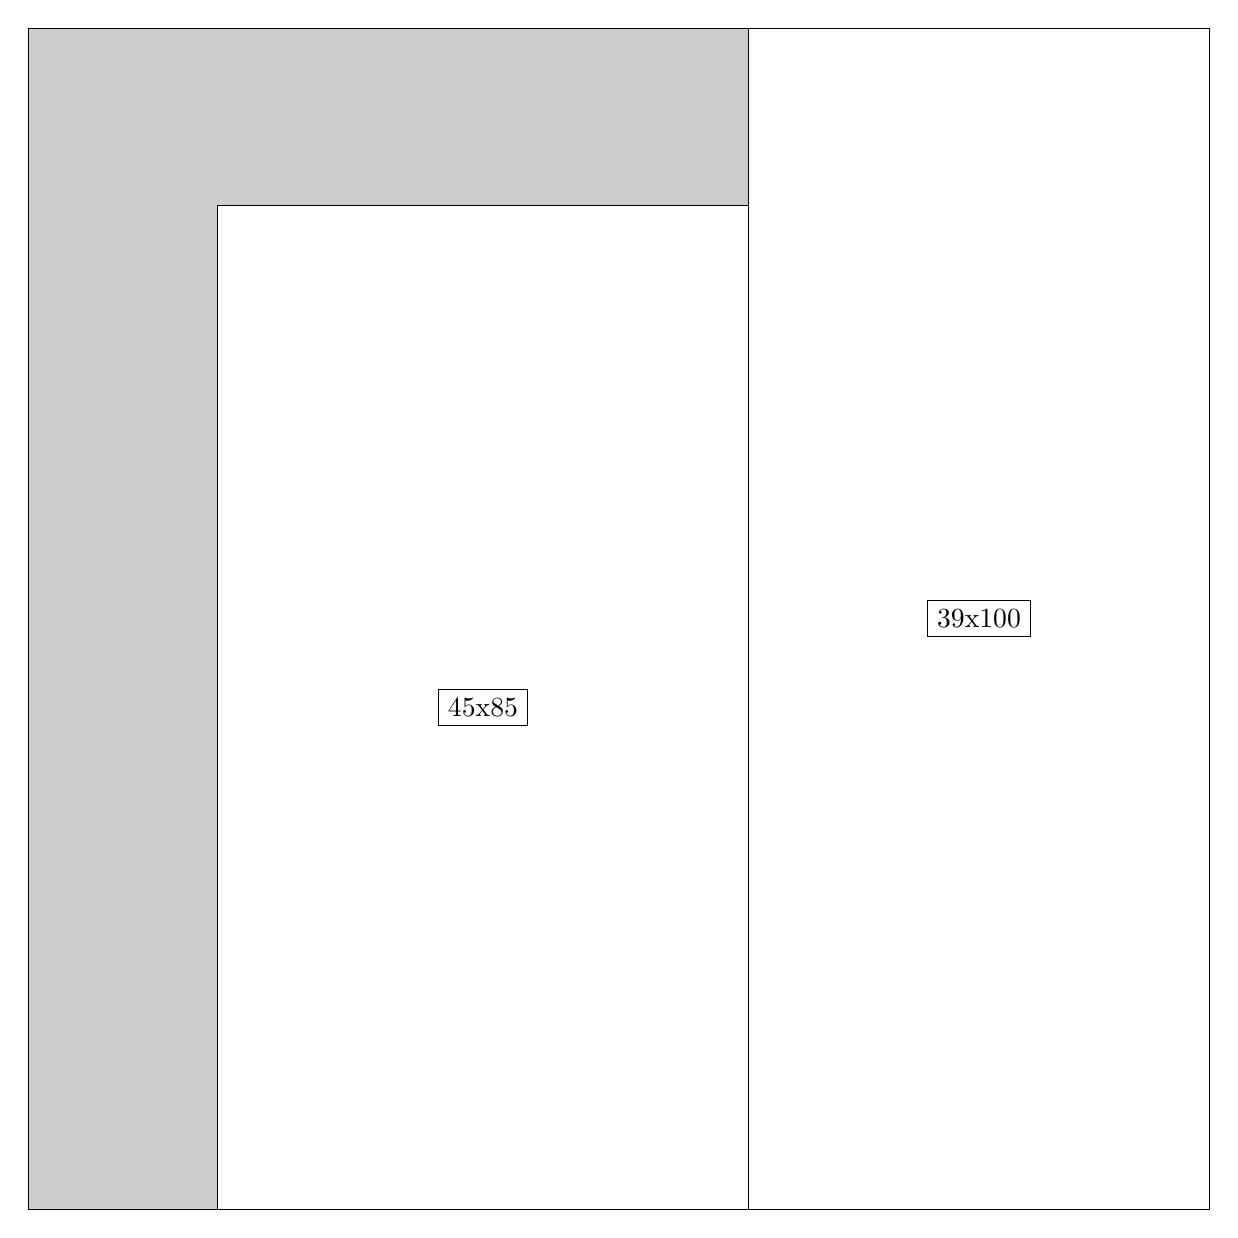
\begin{tikzpicture}[shorten >=1pt,scale=1.0,every node/.style={scale=1.0},->]
\tikzstyle{vertex}=[circle,fill=black!25,minimum size=14pt,inner sep=0pt]
\filldraw[fill=gray!40!white, draw=black] (0,0) rectangle (15.0,15.0);
\foreach \name/\x/\y/\w/\h in {39x100/9.15/0.0/5.85/15.0,45x85/2.4/0.0/6.75/12.75}
\filldraw[fill=white!40!white, draw=black] (\x,\y) rectangle node[draw] (\name) {\name} ++(\w,\h);
\end{tikzpicture}


w =39 , h =100 , x =61 , y =0 , v =3900
\par
w =45 , h =85 , x =16 , y =0 , v =3825
\par
\newpage



\begin{tikzpicture}[shorten >=1pt,scale=1.0,every node/.style={scale=1.0},->]
\tikzstyle{vertex}=[circle,fill=black!25,minimum size=14pt,inner sep=0pt]
\filldraw[fill=gray!40!white, draw=black] (0,0) rectangle (15.0,15.0);
\foreach \name/\x/\y/\w/\h in {65x99/5.25/0.0/9.75/14.85}
\filldraw[fill=white!40!white, draw=black] (\x,\y) rectangle node[draw] (\name) {\name} ++(\w,\h);
\end{tikzpicture}


w =65 , h =99 , x =35 , y =0 , v =6435
\par
\newpage


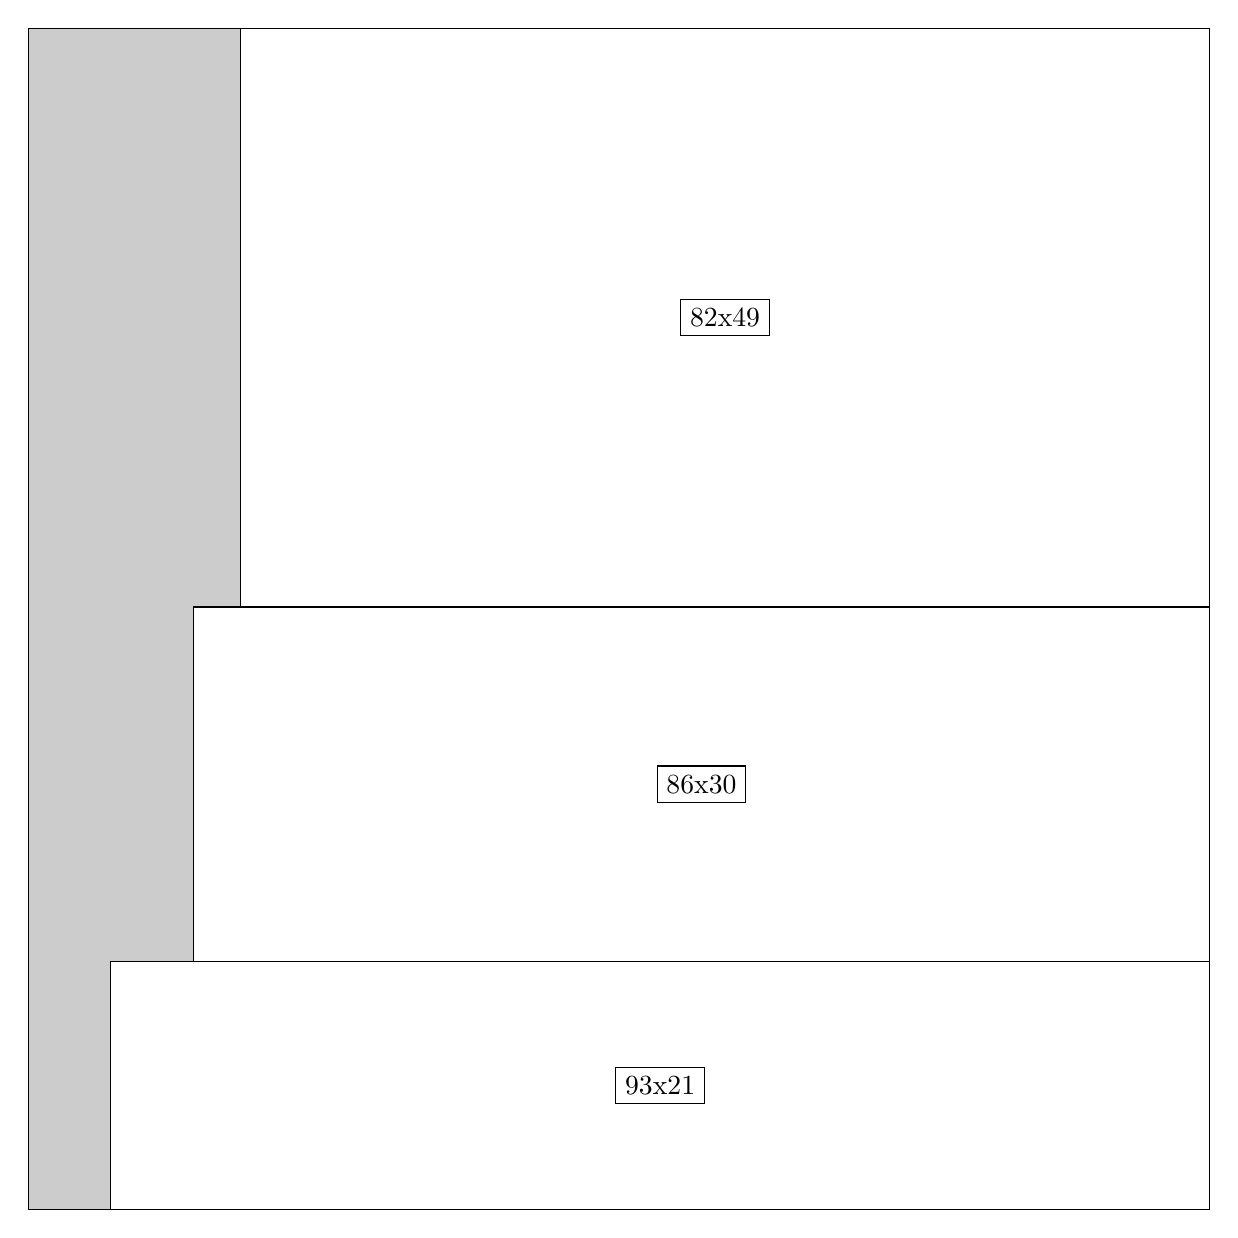
\begin{tikzpicture}[shorten >=1pt,scale=1.0,every node/.style={scale=1.0},->]
\tikzstyle{vertex}=[circle,fill=black!25,minimum size=14pt,inner sep=0pt]
\filldraw[fill=gray!40!white, draw=black] (0,0) rectangle (15.0,15.0);
\foreach \name/\x/\y/\w/\h in {93x21/1.05/0.0/13.95/3.15,86x30/2.1/3.15/12.9/4.5,82x49/2.6999999999999997/7.6499999999999995/12.299999999999999/7.35}
\filldraw[fill=white!40!white, draw=black] (\x,\y) rectangle node[draw] (\name) {\name} ++(\w,\h);
\end{tikzpicture}


w =93 , h =21 , x =7 , y =0 , v =1953
\par
w =86 , h =30 , x =14 , y =21 , v =2580
\par
w =82 , h =49 , x =18 , y =51 , v =4018
\par
\newpage


\end{document}